%%%%%%%%%%%%%%%%%%%%%%%%%%%%%%%%%%%%%%%%%
% Masters/Doctoral Thesis
% LaTeX Template
% Version 2.5 (27/8/17)
%
% This template was downloaded from:
% http://www.LaTeXTemplates.com
%
% Version 2.x major modifications by:
% Vel (vel@latextemplates.com)
%
% This template is based on a template by:
% Steve Gunn (http://users.ecs.soton.ac.uk/srg/softwaretools/document/templates/)
% Sunil Patel (http://www.sunilpatel.co.uk/thesis-template/)
%
% Template license:
% CC BY-NC-SA 3.0 (http://creativecommons.org/licenses/by-nc-sa/3.0/)
%
%%%%%%%%%%%%%%%%%%%%%%%%%%%%%%%%%%%%%%%%%

%----------------------------------------------------------------------------------------
%	PACKAGES AND OTHER DOCUMENT CONFIGURATIONS
%----------------------------------------------------------------------------------------

\documentclass[
	11pt, % The default document font size, options: 10pt, 11pt, 12pt
	%oneside, % Two side (alternating margins) for binding by default, uncomment to switch to one side
	english, % ngerman for German
	singlespacing, % Single line spacing, alternatives: onehalfspacing or doublespacing
	%draft, % Uncomment to enable draft mode (no pictures, no links, overfull hboxes indicated)
	%nolistspacing, % If the document is onehalfspacing or doublespacing, uncomment this to set spacing in lists to single
	liststotoc, % Uncomment to add the list of figures/tables/etc to the table of contents
	toctotoc, % Uncomment to add the main table of contents to the table of contents
	parskip, % Uncomment to add space between paragraphs
	%nohyperref, % Uncomment to not load the hyperref package
	headsepline, % Uncomment to get a line under the header
	chapterinoneline, % Uncomment to place the chapter title next to the number on one line
	% consistentlayout, % Uncomment to change the layout of the declaration, abstract and acknowledgements pages to match the default layout
]{MastersDoctoralThesis} % The class file specifying the document structure

\usepackage[utf8]{inputenc} % Required for inputting international characters
\usepackage[T1]{fontenc} % Output font encoding for international characters

\usepackage{mathpazo} % Use the Palatino font by default

\usepackage[backend=bibtex,style=numeric,natbib=true]{biblatex} % Use the bibtex backend with the authoryear citation style (which resembles APA)

\addbibresource{References.bib} % The filename of the bibliography

\usepackage[autostyle=true]{csquotes} % Required to generate language-dependent quotes in the bibliography

\usepackage[section]{placeins}
\usepackage{float}

\makeatletter

% \AtBeginDocument{
% 	\expandafter\renewcommand\expandafter\subsection\expandafter{
% 		\expandafter\@fb@secFB\subsection
% 	}
% }

\makeatother

\addtocontents{loa}{\def\string\figurename{Algorithm}}

\usepackage{comment}
\usepackage{algorithm}
\usepackage[noend]{algpseudocode}
\usepackage{hyperref}

\usepackage{graphicx}
\def\infinity{\rotatebox{90}{8}}

%----------------------------------------------------------------------------------------
%	MARGIN SETTINGS
%----------------------------------------------------------------------------------------

\geometry{
	paper=a4paper, % Change to letterpaper for US letter
	inner=2.5cm, % Inner margin
	outer=3.8cm, % Outer margin
	bindingoffset=.5cm, % Binding offset
	top=1.5cm, % Top margin
	bottom=1.5cm, % Bottom margin
	%showframe, % Uncomment to show how the type block is set on the page
}

%----------------------------------------------------------------------------------------
%	THESIS INFORMATION
%----------------------------------------------------------------------------------------

\thesistitle{Design and Implementation of AlexNet Deep Learning Network using Reconfigurable Logic} % Your thesis title, this is used in the title and abstract, print it elsewhere with \ttitle
\supervisor{Pr. Apostolos \textsc{Dollas}} % Your supervisor's name, this is used in the title page, print it elsewhere with \supname
\examiner{} % Your examiner's name, this is not currently used anywhere in the template, print it elsewhere with \examname
\degree{Electrical and Computer Engineer} % Your degree name, this is used in the title page and abstract, print it elsewhere with \degreename
\author{Tzanis \textsc{Fotakis}} % Your name, this is used in the title page and abstract, print it elsewhere with \authorname
\addresses{} % Your address, this is not currently used anywhere in the template, print it elsewhere with \addressname

\subject{Electrical and Computer Engineering} % Your subject area, this is not currently used anywhere in the template, print it elsewhere with \subjectname
\keywords{} % Keywords for your thesis, this is not currently used anywhere in the template, print it elsewhere with \keywordnames
\university{\href{https://www.tuc.gr/}{Technical University of Crete}} % Your university's name and URL, this is used in the title page and abstract, print it elsewhere with \univname
\department{\href{https://www.ece.tuc.gr/}{School of Electrical and Computer Engineering}} % Your department's name and URL, this is used in the title page and abstract, print it elsewhere with \deptname
\group{\href{https://www.mhl.tuc.gr/}{Microprocessor and Hardware Laboratory}} % Your research group's name and URL, this is used in the title page, print it elsewhere with \groupname
\faculty{
		% \href{http://faculty.university.com}{Faculty Name}
} % Your faculty's name and URL, this is used in the title page and abstract, print it elsewhere with \facname

\AtBeginDocument{
	\hypersetup{pdftitle=\ttitle} % Set the PDF's title to your title
	\hypersetup{pdfauthor=\authorname} % Set the PDF's author to your name
	\hypersetup{pdfkeywords=\keywordnames} % Set the PDF's keywords to your keywords
}

\begin{document}

\frontmatter % Use roman page numbering style (i, ii, iii, iv...) for the pre-content pages

\pagestyle{plain} % Default to the plain heading style until the thesis style is called for the body content

%----------------------------------------------------------------------------------------
%	TITLE PAGE
%----------------------------------------------------------------------------------------

\begin{titlepage}
	\begin{center}

		\vspace*{.06\textheight}
		{\scshape\LARGE \univname\par}\vspace{1.5cm} % University name
		\textsc{\Large Diploma Thesis}\\[0.5cm] % Thesis type

		\HRule \\[0.4cm] % Horizontal line
		{\huge \bfseries \ttitle\par}\vspace{0.4cm} % Thesis title
		\HRule \\[1.5cm] % Horizontal line

		\begin{minipage}[t]{0.4\textwidth}
			\begin{flushleft} \large
				\emph{Author:}\\
				\href{https://www.linkedin.com/in/fotakistzanis/}{\authorname} % Author name - remove the \href bracket to remove the link
			\end{flushleft}
		\end{minipage}
		\begin{minipage}[t]{0.5\textwidth}
			\begin{flushright} \large
				\emph{Thesis Committee:} \\
				\href{https://www.ece.tuc.gr/index.php?id=4531&tx_tuclabspersonnel_list%5Bperson%5D=289&tx_tuclabspersonnel_list%5Baction%5D=person&tx_tuclabspersonnel_list%5Bcontroller%5D=List}{Prof. Apostolos \textsc{Dollas}}\\ % Supervisor name - remove the \href bracket to remove the link
				\href{https://www.ece.tuc.gr/index.php?id=4531&tx_tuclabspersonnel_list%5Bperson%5D=313&tx_tuclabspersonnel_list%5Baction%5D=person&tx_tuclabspersonnel_list%5Bcontroller%5D=List}{Prof. Michail \textsc{Lagoudakis}}\\
				\href{https://www.linkedin.com/in/christos-kozanitis-a3b173a8/}{Dr. Christos \textsc{Kozanitis}}
			\end{flushright}
		\end{minipage}\\[0.2cm]

		
\includegraphics[scale=0.21]{Images/TUC_logo.png} % University/department logo - uncomment to place it
		\\[0.5cm]

		\vfill

		\large \textit{A thesis submitted in fulfillment of the requirements\\ for the diploma of \degreename}\\[0.3cm] % University requirement text
		\textit{in the}\\[0.4cm]
		\deptname\\\groupname\\[2cm] % Research group name and department name

		\vfill

		{\large \today}\\[4cm] % Date
		%\includegraphics{Logo} % University/department logo - uncomment to place it

		\vfill
	\end{center}
\end{titlepage}

%----------------------------------------------------------------------------------------
%	DECLARATION PAGE
%----------------------------------------------------------------------------------------

\begin{comment}
\begin{declaration}
	\addchaptertocentry{\authorshipname} % Add the declaration to the table of contents
	\noindent I, \authorname, declare that this thesis titled, \enquote{\ttitle} and the work presented in it are my own. I confirm that:

	\begin{itemize}
		\item This work was done wholly or mainly while in candidature for a research degree at this University.
		\item Where any part of this thesis has previously been submitted for a degree or any other qualification at this University or any other institution, this has been clearly stated.
		\item Where I have consulted the published work of others, this is always clearly attributed.
		\item Where I have quoted from the work of others, the source is always given. With the exception of such quotations, this thesis is entirely my own work.
		\item I have acknowledged all main sources of help.
		\item Where the thesis is based on work done by myself jointly with others, I have made clear exactly what was done by others and what I have contributed myself.\\
	\end{itemize}

	\noindent Signed:\\
	\rule[0.5em]{25em}{0.5pt} % This prints a line for the signature

	\noindent Date:\\
	\rule[0.5em]{25em}{0.5pt} % This prints a line to write the date
\end{declaration}

\cleardoublepage
\end{comment}

%----------------------------------------------------------------------------------------
%	QUOTATION PAGE
%----------------------------------------------------------------------------------------

\begin{comment}
\vspace*{0.2\textheight}

\noindent\enquote{\itshape Thanks to my solid academic training, today I can write hundreds of words on virtually any topic without possessing a shred of information, which is how I got a good job in journalism.}\bigbreak

\hfill Dave Barry
\end{comment}

%----------------------------------------------------------------------------------------
%	ABSTRACT PAGE
%----------------------------------------------------------------------------------------

\begin{abstract}
	\addchaptertocentry{\abstractname} % Add the abstract to the table of contents
	% Todo: Add Abstract
	The Thesis Abstract is written here (and usually kept to just this page). The page is kept centered vertically so can expand into the blank space above the title too\ldots
\end{abstract}

%----------------------------------------------------------------------------------------
%	ACKNOWLEDGEMENTS
%----------------------------------------------------------------------------------------

\begin{acknowledgements}
	\addchaptertocentry{\acknowledgementname} % Add the acknowledgements to the table of contents
	% Todo: Add Acknowledgements
	The acknowledgments and the people to thank go here, don't forget to include your project advisor\ldots
\end{acknowledgements}

%----------------------------------------------------------------------------------------
%	LIST OF CONTENTS/FIGURES/TABLES PAGES
%----------------------------------------------------------------------------------------

\tableofcontents % Prints the main table of contents

\listoffigures % Prints the list of figures

\listoftables % Prints the list of tables

\listofalgorithms % Prints the list of algorithms
\addcontentsline{toc}{chapter}{List of Algorithms}

%----------------------------------------------------------------------------------------
%	ABBREVIATIONS
%----------------------------------------------------------------------------------------

% spell-checker: disable
\begin{abbreviations}{ll} % Include a list of abbreviations (a table of two columns)

	\textbf{AI}		& \textbf{A}rtificial \textbf{I}ntelligence\\
	\textbf{ANN}	& \textbf{A}rtificial \textbf{N}eural \textbf{N}etwork\\
	\textbf{ASIC}	& \textbf{A}pplication \textbf{S}pecific \textbf{I}ntegrated \textbf{C}ircuit\\
	\textbf{B-RAM}	& \textbf{B}lock \textbf{R}andom \textbf{A}ccess \textbf{M}emory\\
	\textbf{CNN}	& \textbf{C}onvolutional \textbf{N}eural \textbf{N}etwork\\
	\textbf{CPU}	& \textbf{C}entral \textbf{P}rocessor \textbf{U}nit\\
	\textbf{CS}		& \textbf{C}omputer \textbf{S}cience\\
	\textbf{DDR4}	& \textbf{D}ouble \textbf{D}ata \textbf{R}ate type texbf{4} memory\\
	\textbf{D-RAM}	& \textbf{D}ynamic \textbf{R}andom \textbf{A}ccess \textbf{M}emory\\
	\textbf{DNN}	& \textbf{D}eep \textbf{N}eural \textbf{N}etwork\\
	\textbf{DP}		& \textbf{D}eep \textbf{L}earning\\
	\textbf{DSP}	& \textbf{D}igital \textbf{S}ignal \textbf{P}rocessor\\
	\textbf{FC}		& \textbf{F}ully \textbf{C}onnected\\
	\textbf{FF}		& \textbf{F}lip \textbf{F}lops\\
	\textbf{FPGA}	& \textbf{F}ield \textbf{P}rogrammable \textbf{G}ate \textbf{A}rray\\
	\textbf{FORTH}	& \textbf{F}undation of \textbf{R}esearch and \textbf{T}echnology \textbf{H}ellas\\
	\textbf{GDDR6}	& \textbf{G}raphics \textbf{D}ouble \textbf{D}ata \textbf{R}ate type \textbf{6} memory\\
	\textbf{GPU}	& \textbf{G}raphic \textbf{P}rocessor \textbf{U}nit\\
	\textbf{HBM}	& \textbf{H}igh \textbf{B}andwidth \textbf{M}emory\\
	\textbf{HLS}	& \textbf{H}igh \textbf{L}evel \textbf{S}ynthesis\\
	\textbf{HPC}	& \textbf{H}ight \textbf{P}erformance \textbf{C}omputing\\
	\textbf{LUT}	& \textbf{L}ook \textbf{U}p \textbf{T}able\\
	\textbf{ML}		& \textbf{M}achine \textbf{L}earning\\
	\textbf{MPSoC}	& \textbf{M}ulti \textbf{P}rocessor \textbf{S}ystem \textbf{o}n \textbf{C}hip\\
	\textbf{QFDB}	& \textbf{Q}uad \textbf{F}PGA \textbf{D}aughter \textbf{B}oard\\
	\textbf{RAM}	& \textbf{R}andom Access Memory\\
	\textbf{ReLU}	& \textbf{R}ectified \textbf{L}inear \textbf{U}nit\\
	\textbf{SDK}	& \textbf{S}oftware \textbf{D}evelopment \textbf{K}it\\
	\textbf{SLC}	& \textbf{S}econd \textbf{L}evel \textbf{C}odebook\\
	\textbf{SSD}	& \textbf{S}olid \textbf{S}tate \textbf{D}rive\\
	\textbf{TDP}	& \textbf{T}hermal \textbf{D}esign \textbf{P}ower\\
	\textbf{TPU}	& \textbf{T}ensor \textbf{P}rocessor \textbf{U}nit\\
	\textbf{USD}	& \textbf{U}nited \textbf{S}tates \textbf{D}ollar\\

\end{abbreviations}
% spell-checker: enable

%----------------------------------------------------------------------------------------
%	PHYSICAL CONSTANTS/OTHER DEFINITIONS
%----------------------------------------------------------------------------------------

\begin{comment}
\begin{constants}{lr@{${}={}$}l} % The list of physical constants is a three column table

	% The \SI{}{} command is provided by the siunitx package, see its documentation for instructions on how to use it

	Speed of Light & $c_{0}$ & \SI{2.99792458e8}{\meter\per\second} (exact)\\
	%Constant Name & $Symbol$ & $Constant Value$ with units\\

\end{constants}
\end{comment}

%----------------------------------------------------------------------------------------
%	SYMBOLS
%----------------------------------------------------------------------------------------

\begin{comment}
\begin{symbols}{lll} % Include a list of Symbols (a three column table)

	$a$ & distance & \si{\meter} \\
	$P$ & power & \si{\watt} (\si{\joule\per\second}) \\
	%Symbol & Name & Unit \\

	\addlinespace % Gap to separate the Roman symbols from the Greek

	$\omega$ & angular frequency & \si{\radian} \\

\end{symbols}
\end{comment}

%----------------------------------------------------------------------------------------
%	DEDICATION
%----------------------------------------------------------------------------------------

\dedicatory{Dedicated to my family and friends\ldots}

%----------------------------------------------------------------------------------------
%	THESIS CONTENT - CHAPTERS
%----------------------------------------------------------------------------------------

\mainmatter % Begin numeric (1,2,3...) page numbering

\pagestyle{thesis} % Return the page headers back to the "thesis" style

% Include the chapters of the thesis as separate files from the Chapters folder
% Uncomment the lines as you write the chapters

% Chapter 1

\chapter{Chapter Title Here} % Main chapter title

\label{Chapter1} % For referencing the chapter elsewhere, use \ref{Chapter1}

%----------------------------------------------------------------------------------------

% Define some commands to keep the formatting separated from the content
\newcommand{\keyword}[1]{\textbf{#1}}
\newcommand{\tabhead}[1]{\textbf{#1}}
\newcommand{\code}[1]{\texttt{#1}}
\newcommand{\file}[1]{\texttt{\bfseries#1}}
\newcommand{\option}[1]{\texttt{\itshape#1}}

%----------------------------------------------------------------------------------------

\section{Welcome and Thank You}
Welcome to this \LaTeX{} Thesis Template, a beautiful and easy to use template for writing a thesis using the \LaTeX{} typesetting system.

If you are writing a thesis (or will be in the future) and its subject is technical or mathematical (though it doesn't have to be), then creating it in \LaTeX{} is highly recommended as a way to make sure you can just get down to the essential writing without having to worry over formatting or wasting time arguing with your word processor.

\LaTeX{} is easily able to professionally typeset documents that run to hundreds or thousands of pages long. With simple mark-up commands, it automatically sets out the table of contents, margins, page headers and footers and keeps the formatting consistent and beautiful. One of its main strengths is the way it can easily typeset mathematics, even \emph{heavy} mathematics. Even if those equations are the most horribly twisted and most difficult mathematical problems that can only be solved on a super-computer, you can at least count on \LaTeX{} to make them look stunning.

%----------------------------------------------------------------------------------------

\section{Learning \LaTeX{}}

\LaTeX{} is not a \textsc{wysiwyg} (What You See is What You Get) program, unlike word processors such as Microsoft Word or Apple's Pages. Instead, a document written for \LaTeX{} is actually a simple, plain text file that contains \emph{no formatting}. You tell \LaTeX{} how you want the formatting in the finished document by writing in simple commands amongst the text, for example, if I want to use \emph{italic text for emphasis}, I write the \verb|\emph{text}| command and put the text I want in italics in between the curly braces. This means that \LaTeX{} is a \enquote{mark-up} language, very much like HTML.

\subsection{A (not so short) Introduction to \LaTeX{}}

If you are new to \LaTeX{}, there is a very good eBook -- freely available online as a PDF file -- called, \enquote{The Not So Short Introduction to \LaTeX{}}. The book's title is typically shortened to just \emph{lshort}. You can download the latest version (as it is occasionally updated) from here:
\url{http://www.ctan.org/tex-archive/info/lshort/english/lshort.pdf}

It is also available in several other languages. Find yours from the list on this page: \url{http://www.ctan.org/tex-archive/info/lshort/}

It is recommended to take a little time out to learn how to use \LaTeX{} by creating several, small `test' documents, or having a close look at several templates on:\\
\url{http://www.LaTeXTemplates.com}\\
Making the effort now means you're not stuck learning the system when what you \emph{really} need to be doing is writing your thesis.

\subsection{A Short Math Guide for \LaTeX{}}

If you are writing a technical or mathematical thesis, then you may want to read the document by the AMS (American Mathematical Society) called, \enquote{A Short Math Guide for \LaTeX{}}. It can be found online here:
\url{http://www.ams.org/tex/amslatex.html}
under the \enquote{Additional Documentation} section towards the bottom of the page.

\subsection{Common \LaTeX{} Math Symbols}
There are a multitude of mathematical symbols available for \LaTeX{} and it would take a great effort to learn the commands for them all. The most common ones you are likely to use are shown on this page:
\url{http://www.sunilpatel.co.uk/latex-type/latex-math-symbols/}

You can use this page as a reference or crib sheet, the symbols are rendered as large, high quality images so you can quickly find the \LaTeX{} command for the symbol you need.

\subsection{\LaTeX{} on a Mac}

The \LaTeX{} distribution is available for many systems including Windows, Linux and Mac OS X. The package for OS X is called MacTeX and it contains all the applications you need -- bundled together and pre-customized -- for a fully working \LaTeX{} environment and work flow.

MacTeX includes a custom dedicated \LaTeX{} editor called TeXShop for writing your `\file{.tex}' files and BibDesk: a program to manage your references and create your bibliography section just as easily as managing songs and creating playlists in iTunes.

%----------------------------------------------------------------------------------------

\section{Getting Started with this Template}

If you are familiar with \LaTeX{}, then you should explore the directory structure of the template and then proceed to place your own information into the \emph{THESIS INFORMATION} block of the \file{main.tex} file. You can then modify the rest of this file to your unique specifications based on your degree/university. Section \ref{FillingFile} on page \pageref{FillingFile} will help you do this. Make sure you also read section \ref{ThesisConventions} about thesis conventions to get the most out of this template.

If you are new to \LaTeX{} it is recommended that you carry on reading through the rest of the information in this document.

Before you begin using this template you should ensure that its style complies with the thesis style guidelines imposed by your institution. In most cases this template style and layout will be suitable. If it is not, it may only require a small change to bring the template in line with your institution's recommendations. These modifications will need to be done on the \file{MastersDoctoralThesis.cls} file.

\subsection{About this Template}

This \LaTeX{} Thesis Template is originally based and created around a \LaTeX{} style file created by Steve R.\ Gunn from the University of Southampton (UK), department of Electronics and Computer Science. You can find his original thesis style file at his site, here:
\url{http://www.ecs.soton.ac.uk/~srg/softwaretools/document/templates/}

Steve's \file{ecsthesis.cls} was then taken by Sunil Patel who modified it by creating a skeleton framework and folder structure to place the thesis files in. The resulting template can be found on Sunil's site here:
\url{http://www.sunilpatel.co.uk/thesis-template}

Sunil's template was made available through \url{http://www.LaTeXTemplates.com} where it was modified many times based on user requests and questions. Version 2.0 and onwards of this template represents a major modification to Sunil's template and is, in fact, hardly recognisable. The work to make version 2.0 possible was carried out by \href{mailto:vel@latextemplates.com}{Vel} and Johannes Böttcher.

%----------------------------------------------------------------------------------------

\section{What this Template Includes}

\subsection{Folders}

This template comes as a single zip file that expands out to several files and folders. The folder names are mostly self-explanatory:

\keyword{Appendices} -- this is the folder where you put the appendices. Each appendix should go into its own separate \file{.tex} file. An example and template are included in the directory.

\keyword{Chapters} -- this is the folder where you put the thesis chapters. A thesis usually has about six chapters, though there is no hard rule on this. Each chapter should go in its own separate \file{.tex} file and they can be split as:
\begin{itemize}
	\item Chapter 1: Introduction to the thesis topic
	\item Chapter 2: Background information and theory
	\item Chapter 3: (Laboratory) experimental setup
	\item Chapter 4: Details of experiment 1
	\item Chapter 5: Details of experiment 2
	\item Chapter 6: Discussion of the experimental results
	\item Chapter 7: Conclusion and future directions
\end{itemize}
This chapter layout is specialised for the experimental sciences, your discipline may be different.

\keyword{Figures} -- this folder contains all figures for the thesis. These are the final images that will go into the thesis document.

\subsection{Files}

Included are also several files, most of them are plain text and you can see their contents in a text editor. After initial compilation, you will see that more auxiliary files are created by \LaTeX{} or BibTeX and which you don't need to delete or worry about:

\keyword{example.bib} -- this is an important file that contains all the bibliographic information and references that you will be citing in the thesis for use with BibTeX. You can write it manually, but there are reference manager programs available that will create and manage it for you. Bibliographies in \LaTeX{} are a large subject and you may need to read about BibTeX before starting with this. Many modern reference managers will allow you to export your references in BibTeX format which greatly eases the amount of work you have to do.

\keyword{MastersDoctoralThesis.cls} -- this is an important file. It is the class file that tells \LaTeX{} how to format the thesis.

\keyword{main.pdf} -- this is your beautifully typeset thesis (in the PDF file format) created by \LaTeX{}. It is supplied in the PDF with the template and after you compile the template you should get an identical version.

\keyword{main.tex} -- this is an important file. This is the file that you tell \LaTeX{} to compile to produce your thesis as a PDF file. It contains the framework and constructs that tell \LaTeX{} how to layout the thesis. It is heavily commented so you can read exactly what each line of code does and why it is there. After you put your own information into the \emph{THESIS INFORMATION} block -- you have now started your thesis!

Files that are \emph{not} included, but are created by \LaTeX{} as auxiliary files include:

\keyword{main.aux} -- this is an auxiliary file generated by \LaTeX{}, if it is deleted \LaTeX{} simply regenerates it when you run the main \file{.tex} file.

\keyword{main.bbl} -- this is an auxiliary file generated by BibTeX, if it is deleted, BibTeX simply regenerates it when you run the \file{main.aux} file. Whereas the \file{.bib} file contains all the references you have, this \file{.bbl} file contains the references you have actually cited in the thesis and is used to build the bibliography section of the thesis.

\keyword{main.blg} -- this is an auxiliary file generated by BibTeX, if it is deleted BibTeX simply regenerates it when you run the main \file{.aux} file.

\keyword{main.lof} -- this is an auxiliary file generated by \LaTeX{}, if it is deleted \LaTeX{} simply regenerates it when you run the main \file{.tex} file. It tells \LaTeX{} how to build the \emph{List of Figures} section.

\keyword{main.log} -- this is an auxiliary file generated by \LaTeX{}, if it is deleted \LaTeX{} simply regenerates it when you run the main \file{.tex} file. It contains messages from \LaTeX{}, if you receive errors and warnings from \LaTeX{}, they will be in this \file{.log} file.

\keyword{main.lot} -- this is an auxiliary file generated by \LaTeX{}, if it is deleted \LaTeX{} simply regenerates it when you run the main \file{.tex} file. It tells \LaTeX{} how to build the \emph{List of Tables} section.

\keyword{main.out} -- this is an auxiliary file generated by \LaTeX{}, if it is deleted \LaTeX{} simply regenerates it when you run the main \file{.tex} file.

So from this long list, only the files with the \file{.bib}, \file{.cls} and \file{.tex} extensions are the most important ones. The other auxiliary files can be ignored or deleted as \LaTeX{} and BibTeX will regenerate them.

%----------------------------------------------------------------------------------------

\section{Filling in Your Information in the \file{main.tex} File}\label{FillingFile}

You will need to personalize the thesis template and make it your own by filling in your own information. This is done by editing the \file{main.tex} file in a text editor or your favorite LaTeX environment.

Open the file and scroll down to the third large block titled \emph{THESIS INFORMATION} where you can see the entries for \emph{University Name}, \emph{Department Name}, etc \ldots

Fill out the information about yourself, your group and institution. You can also insert web links, if you do, make sure you use the full URL, including the \code{http://} for this. If you don't want these to be linked, simply remove the \verb|\href{url}{name}| and only leave the name.

When you have done this, save the file and recompile \code{main.tex}. All the information you filled in should now be in the PDF, complete with web links. You can now begin your thesis proper!

%----------------------------------------------------------------------------------------

\section{The \code{main.tex} File Explained}

The \file{main.tex} file contains the structure of the thesis. There are plenty of written comments that explain what pages, sections and formatting the \LaTeX{} code is creating. Each major document element is divided into commented blocks with titles in all capitals to make it obvious what the following bit of code is doing. Initially there seems to be a lot of \LaTeX{} code, but this is all formatting, and it has all been taken care of so you don't have to do it.

Begin by checking that your information on the title page is correct. For the thesis declaration, your institution may insist on something different than the text given. If this is the case, just replace what you see with what is required in the \emph{DECLARATION PAGE} block.

Then comes a page which contains a funny quote. You can put your own, or quote your favorite scientist, author, person, and so on. Make sure to put the name of the person who you took the quote from.

Following this is the abstract page which summarizes your work in a condensed way and can almost be used as a standalone document to describe what you have done. The text you write will cause the heading to move up so don't worry about running out of space.

Next come the acknowledgements. On this page, write about all the people who you wish to thank (not forgetting parents, partners and your advisor/supervisor).

The contents pages, list of figures and tables are all taken care of for you and do not need to be manually created or edited. The next set of pages are more likely to be optional and can be deleted since they are for a more technical thesis: insert a list of abbreviations you have used in the thesis, then a list of the physical constants and numbers you refer to and finally, a list of mathematical symbols used in any formulae. Making the effort to fill these tables means the reader has a one-stop place to refer to instead of searching the internet and references to try and find out what you meant by certain abbreviations or symbols.

The list of symbols is split into the Roman and Greek alphabets. Whereas the abbreviations and symbols ought to be listed in alphabetical order (and this is \emph{not} done automatically for you) the list of physical constants should be grouped into similar themes.

The next page contains a one line dedication. Who will you dedicate your thesis to?

Finally, there is the block where the chapters are included. Uncomment the lines (delete the \code{\%} character) as you write the chapters. Each chapter should be written in its own file and put into the \emph{Chapters} folder and named \file{Chapter1}, \file{Chapter2}, etc\ldots Similarly for the appendices, uncomment the lines as you need them. Each appendix should go into its own file and placed in the \emph{Appendices} folder.

After the preamble, chapters and appendices finally comes the bibliography. The bibliography style (called \option{authoryear}) is used for the bibliography and is a fully featured style that will even include links to where the referenced paper can be found online. Do not underestimate how grateful your reader will be to find that a reference to a paper is just a click away. Of course, this relies on you putting the URL information into the BibTeX file in the first place.

%----------------------------------------------------------------------------------------

\section{Thesis Features and Conventions}\label{ThesisConventions}

To get the best out of this template, there are a few conventions that you may want to follow.

One of the most important (and most difficult) things to keep track of in such a long document as a thesis is consistency. Using certain conventions and ways of doing things (such as using a Todo list) makes the job easier. Of course, all of these are optional and you can adopt your own method.

\subsection{Printing Format}

This thesis template is designed for double sided printing (i.e. content on the front and back of pages) as most theses are printed and bound this way. Switching to one sided printing is as simple as uncommenting the \option{oneside} option of the \code{documentclass} command at the top of the \file{main.tex} file. You may then wish to adjust the margins to suit specifications from your institution.

The headers for the pages contain the page number on the outer side (so it is easy to flick through to the page you want) and the chapter name on the inner side.

The text is set to 11 point by default with single line spacing, again, you can tune the text size and spacing should you want or need to using the options at the very start of \file{main.tex}. The spacing can be changed similarly by replacing the \option{singlespacing} with \option{onehalfspacing} or \option{doublespacing}.

\subsection{Using US Letter Paper}

The paper size used in the template is A4, which is the standard size in Europe. If you are using this thesis template elsewhere and particularly in the United States, then you may have to change the A4 paper size to the US Letter size. This can be done in the margins settings section in \file{main.tex}.

Due to the differences in the paper size, the resulting margins may be different to what you like or require (as it is common for institutions to dictate certain margin sizes). If this is the case, then the margin sizes can be tweaked by modifying the values in the same block as where you set the paper size. Now your document should be set up for US Letter paper size with suitable margins.

\subsection{References}

The \code{biblatex} package is used to format the bibliography and inserts references such as this one \parencite{Reference1}. The options used in the \file{main.tex} file mean that the in-text citations of references are formatted with the author(s) listed with the date of the publication. Multiple references are separated by semicolons (e.g. \parencite{Reference2, Reference1}) and references with more than three authors only show the first author with \emph{et al.} indicating there are more authors (e.g. \parencite{Reference3}). This is done automatically for you. To see how you use references, have a look at the \file{Chapter1.tex} source file. Many reference managers allow you to simply drag the reference into the document as you type.

Scientific references should come \emph{before} the punctuation mark if there is one (such as a comma or period). The same goes for footnotes\footnote{Such as this footnote, here down at the bottom of the page.}. You can change this but the most important thing is to keep the convention consistent throughout the thesis. Footnotes themselves should be full, descriptive sentences (beginning with a capital letter and ending with a full stop). The APA6 states: \enquote{Footnote numbers should be superscripted, [...], following any punctuation mark except a dash.} The Chicago manual of style states: \enquote{A note number should be placed at the end of a sentence or clause. The number follows any punctuation mark except the dash, which it precedes. It follows a closing parenthesis.}

The bibliography is typeset with references listed in alphabetical order by the first author's last name. This is similar to the APA referencing style. To see how \LaTeX{} typesets the bibliography, have a look at the very end of this document (or just click on the reference number links in in-text citations).

\subsubsection{A Note on bibtex}

The bibtex backend used in the template by default does not correctly handle unicode character encoding (i.e. "international" characters). You may see a warning about this in the compilation log and, if your references contain unicode characters, they may not show up correctly or at all. The solution to this is to use the biber backend instead of the outdated bibtex backend. This is done by finding this in \file{main.tex}: \option{backend=bibtex} and changing it to \option{backend=biber}. You will then need to delete all auxiliary BibTeX files and navigate to the template directory in your terminal (command prompt). Once there, simply type \code{biber main} and biber will compile your bibliography. You can then compile \file{main.tex} as normal and your bibliography will be updated. An alternative is to set up your LaTeX editor to compile with biber instead of bibtex, see \href{http://tex.stackexchange.com/questions/154751/biblatex-with-biber-configuring-my-editor-to-avoid-undefined-citations/}{here} for how to do this for various editors.

\subsection{Tables}

Tables are an important way of displaying your results, below is an example table which was generated with this code:

{\small
\begin{verbatim}
\begin{table}
\caption{The effects of treatments X and Y on the four groups studied.}
\label{tab:treatments}
\centering
\begin{tabular}{l l l}
\toprule
\tabhead{Groups} & \tabhead{Treatment X} & \tabhead{Treatment Y} \\
\midrule
1 & 0.2 & 0.8\\
2 & 0.17 & 0.7\\
3 & 0.24 & 0.75\\
4 & 0.68 & 0.3\\
\bottomrule
\end{tabular}
\end{table}
\end{verbatim}
}

\begin{table}
	\caption{The effects of treatments X and Y on the four groups studied.}
	\label{tab:treatments}
	\centering
	\begin{tabular}{l l l}
		\toprule
		\tabhead{Groups} & \tabhead{Treatment X} & \tabhead{Treatment Y} \\
		\midrule
		1                & 0.2                   & 0.8                   \\
		2                & 0.17                  & 0.7                   \\
		3                & 0.24                  & 0.75                  \\
		4                & 0.68                  & 0.3                   \\
		\bottomrule                                                      \\
	\end{tabular}
\end{table}

You can reference tables with \verb|\ref{<label>}| where the label is defined within the table environment. See \file{Chapter1.tex} for an example of the label and citation (e.g. Table~\ref{tab:treatments}).

\subsection{Figures}

There will hopefully be many figures in your thesis (that should be placed in the \emph{Figures} folder). The way to insert figures into your thesis is to use a code template like this:
\begin{verbatim}
\begin{figure}
\centering
\includegraphics{Figures/Electron}
\decoRule
\caption[An Electron]{An electron (artist's impression).}
\label{fig:Electron}
\end{figure}
\end{verbatim}
Also look in the source file. Putting this code into the source file produces the picture of the electron that you can see in the figure below.

\begin{figure}[th]
	\centering
	\includegraphics{Figures/Electron}
	\decoRule
	\caption[An Electron]{An electron (artist's impression).}
	\label{fig:Electron}
\end{figure}

Sometimes figures don't always appear where you write them in the source. The placement depends on how much space there is on the page for the figure. Sometimes there is not enough room to fit a figure directly where it should go (in relation to the text) and so \LaTeX{} puts it at the top of the next page. Positioning figures is the job of \LaTeX{} and so you should only worry about making them look good!

Figures usually should have captions just in case you need to refer to them (such as in Figure~\ref{fig:Electron}). The \verb|\caption| command contains two parts, the first part, inside the square brackets is the title that will appear in the \emph{List of Figures}, and so should be short. The second part in the curly brackets should contain the longer and more descriptive caption text.

The \verb|\decoRule| command is optional and simply puts an aesthetic horizontal line below the image. If you do this for one image, do it for all of them.

\LaTeX{} is capable of using images in pdf, jpg and png format.

\subsection{Typesetting mathematics}

If your thesis is going to contain heavy mathematical content, be sure that \LaTeX{} will make it look beautiful, even though it won't be able to solve the equations for you.

The \enquote{Not So Short Introduction to \LaTeX} (available on \href{http://www.ctan.org/tex-archive/info/lshort/english/lshort.pdf}{CTAN}) should tell you everything you need to know for most cases of typesetting mathematics. If you need more information, a much more thorough mathematical guide is available from the AMS called, \enquote{A Short Math Guide to \LaTeX} and can be downloaded from:
\url{ftp://ftp.ams.org/pub/tex/doc/amsmath/short-math-guide.pdf}

There are many different \LaTeX{} symbols to remember, luckily you can find the most common symbols in \href{http://ctan.org/pkg/comprehensive}{The Comprehensive \LaTeX~Symbol List}.

You can write an equation, which is automatically given an equation number by \LaTeX{} like this:
\begin{verbatim}
\begin{equation}
E = mc^{2}
\label{eqn:Einstein}
\end{equation}
\end{verbatim}

This will produce Einstein's famous energy-matter equivalence equation:
\begin{equation}
	E = mc^{2}
	\label{eqn:Einstein}
\end{equation}

All equations you write (which are not in the middle of paragraph text) are automatically given equation numbers by \LaTeX{}. If you don't want a particular equation numbered, use the unnumbered form:
\begin{verbatim}
\[ a^{2}=4 \]
\end{verbatim}

%----------------------------------------------------------------------------------------

\section{Sectioning and Subsectioning}

You should break your thesis up into nice, bite-sized sections and subsections. \LaTeX{} automatically builds a table of Contents by looking at all the \verb|\chapter{}|, \verb|\section{}|  and \verb|\subsection{}| commands you write in the source.

The Table of Contents should only list the sections to three (3) levels. A \verb|chapter{}| is level zero (0). A \verb|\section{}| is level one (1) and so a \verb|\subsection{}| is level two (2). In your thesis it is likely that you will even use a \verb|subsubsection{}|, which is level three (3). The depth to which the Table of Contents is formatted is set within \file{MastersDoctoralThesis.cls}. If you need this changed, you can do it in \file{main.tex}.

%----------------------------------------------------------------------------------------

\section{In Closing}

You have reached the end of this mini-guide. You can now rename or overwrite this pdf file and begin writing your own \file{Chapter1.tex} and the rest of your thesis. The easy work of setting up the structure and framework has been taken care of for you. It's now your job to fill it out!

Good luck and have lots of fun!

\begin{flushright}
	Guide written by ---\\
	Sunil Patel: \href{http://www.sunilpatel.co.uk}{www.sunilpatel.co.uk}\\
	Vel: \href{http://www.LaTeXTemplates.com}{LaTeXTemplates.com}
\end{flushright}

\chapter{Introduction}

\label{Chapter-Introduction}

Since the invention of the first computer, humankind is rapidly solving problems that are intellectually difficult for human beings but relatively easy for computers, as such problems can be described in detail with a formal list of mathematical rules. However, problems that are easy for humans, that are solved intuitively, like distinguishing the difference between a car and a person, or a spoken word and a bird's chirp, is a real challenge for computers and engineers \cite{Goodfellow-et-al-2016}. Those problems cannot be described, at the time of writing, with sharply defined mathematical rules. Artificial Intelligence (AI) and Machine Learning (ML) study those types of problems, with many successes in the cost of highly computationally complex algorithms.

It is estimated that by the year 2025, the total amount of data created worldwide will rise to 163 ZettaBytes, while every minute of the year 2019, Americans used more than 4.4 PetaBytes of data \cite{Forbes-How-Much-Data-Is-Collected-Every-Minute-Of-The-Day}. It is evident that data management systems and knowledge extraction from them, also called Data Analysis, are urgent. Although such problems can be tackled using Artificial Intelligence and Machine Learning, it is extremely computationally intensive, if not even non-feasible, in a reasonable amount of time.

Fortunately, most of the algorithms used to tackle such problems come with high parallelism. Therefore, they can be expanded in the space domain, in other words, they can utilize more hardware resources to cut down on needs from the time domain. Of course, there are many different types of hardware resources, each with their advantages and disadvantages, from parallelism capabilities and energy efficiency to cost of production, reconfigurability, and reusability.

\section{Motivation}
Nowadays, the computational complexity of the aforementioned algorithms makes hardware acceleration a necessity, since running them on Central Processing Units (CPUs) is, while possible, the least efficient and fast solution. Although writing software for CPUs may be fast and easy, its running speed due to low parallelism and high power consumption, as a general propose piece of hardware, are far from ideal. For reference, at the time of writing, a top-grade server CPU, AMD EPYC 7002 Series (Figure \ref{fig:amd-epyc-7002-chip}), can provide up to 64 cores and 128 threads, at up to 2.25GHz base clock and 3.4GHz boost clock, with a rated Thermal Design Power (TDP) of 225Watts, and a list price of 4,425 USD \cite{AMD-EPYC-7002-Series-Processors}.

\begin{figure} [H]
	\centering
	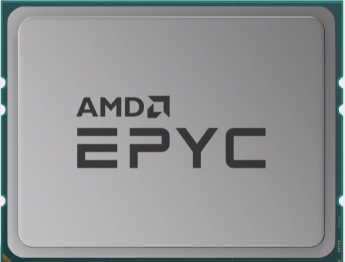
\includegraphics[scale=0.45]{Images/Hardware/amd-epyc.png}
	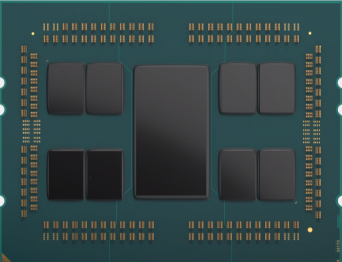
\includegraphics[scale=0.45]{Images/Hardware/amd-epyc-dies.png}
	\decoRule
	\caption[AMD Epyc 7002 series chip]{AMD Epyc 7002 series chip: \href{https://www.amd.com/en/processors/epyc-7002-series}{URL}}
	\label{fig:amd-epyc-7002-chip}
\end{figure}

Graphics Processing Units (GPUs), on the other hand, provide much higher parallelism, while still being relatively easy for their software to be written. However, they can be costly to scale up, and their power consumption can be really high. For reference, at the time of writing, a top-grade GPU for ML, NVIDIA Titan RTX (Figure \ref{fig:nvidia-titan-rtx-explosion-view}), provides up to 72 Streaming Multiprocessors, up to 4,608 CUDA Cores and up to 576 Tensor cores, with a rated base clock of 1,350 MHz and boost clock of 1,770 MHz, 24 GB of Graphics Double Data Rate (GDDR6) Memory and a power consumption of 280 Watts for 2,500 USD \cite{NVIDIA-Titan-RTX-GPU}.

\begin{figure} [H]
	\centering
	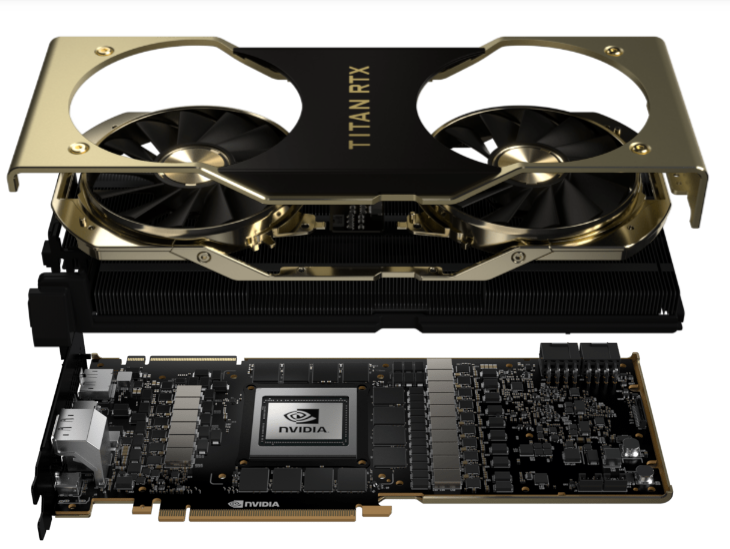
\includegraphics[scale=0.5]{Images/Hardware/NVIDIA-Titan-RTX.png}
	% 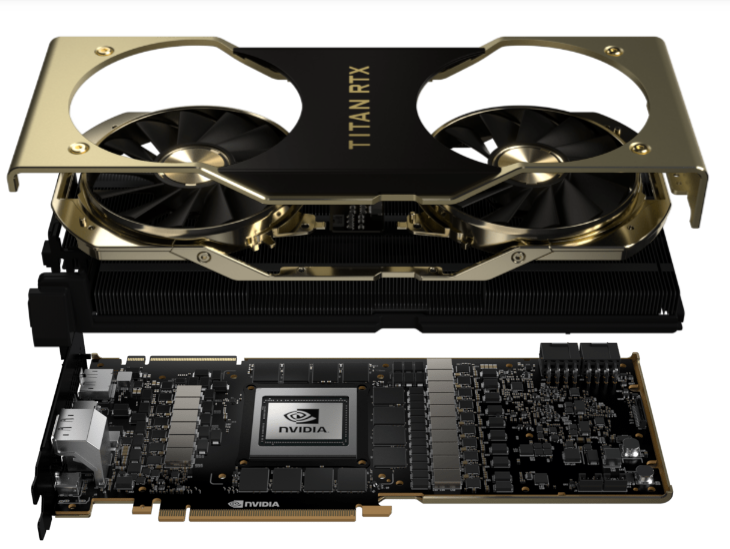
\includegraphics[width=\textwidth]{Images/Hardware/NVIDIA-Titan-RTX.png}
	\decoRule
	\caption[NVIDIA Titan RTX card]{NVIDIA Titan RTX card: \href{https://www.nvidia.com/en-us/deep-learning-ai/products/titan-rtx/}{URL}}
	\label{fig:nvidia-titan-rtx-explosion-view}
\end{figure}

Moreover, there are Application Specific Integrated Circuits (ASICs), which can provide the best parallelism capabilities and the lowest power consumption for a particular application. Unfortunately, they are very expensive to develop and produce, and they can only serve a single purpose, a single application. An example of such an ASIC is the Google Cloud Tensor Processing Unit (TPU) (Figure \ref{fig:google-tpu-motherboard}), which, for the third version (v3), in a single chip there are two TPU cores, each of which contains two scalar, vector, and matrix units (MXUs), and 16 GB of High Bandwidth Memory (HBM) \cite{Google-Cloud-TPU}.

\begin{figure} [H]
	\centering
	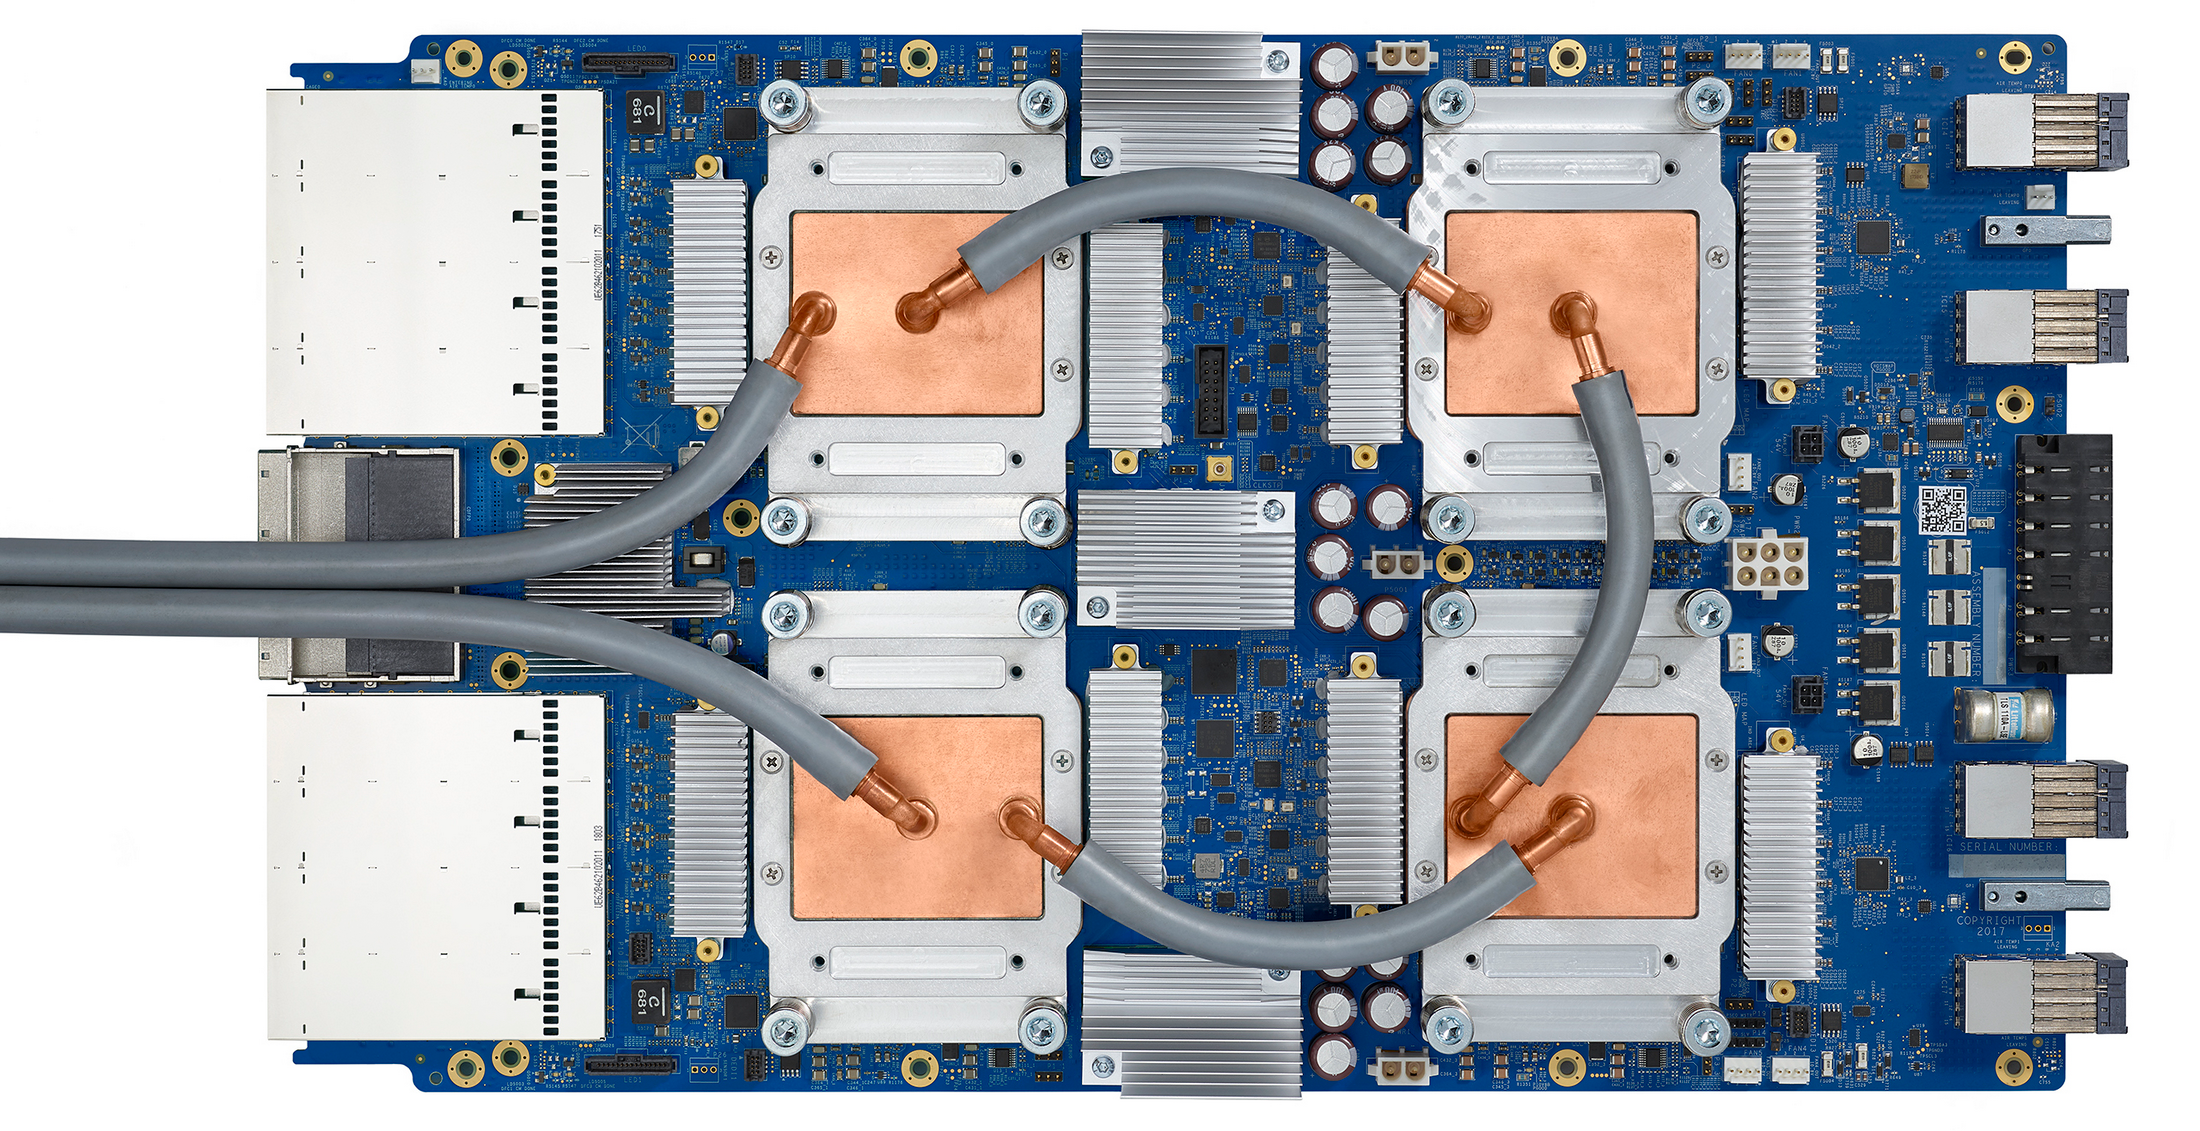
\includegraphics[width=\textwidth]{Images/Hardware/tpu-v3.png}
	\decoRule
	\caption[Google's TPU v3]{Google's TPU v3 - 4 chips, 2 cores per chip: \href{https://cloud.google.com/tpu/docs/system-architecture}{URL}}
	\label{fig:google-tpu-motherboard}
\end{figure}

On the contrary, Field Programmable Gate Arrays (FPGAs) are bridging the gap between the GPUs' flexibility and the ASICs' performance and power consumption. An example FPGA Hardware targeted for High-Performance Computing (HPC) is the Quad-FPGA Daughter Board (QFDB) (Figure \ref{fig:forth-qfdb-daughterboard}) \cite{Implementation-and-Impact-of-an-Ultra-Compact-Multi-FPGA-Board-for-Large-System-Prototyping}, developed by the Foundation of Research and Technology Hellas (FORTH) \cite{FORTH}, combines four interconnected Xilinx Zynq Ultrascale+ Multi-Processor Systems on Chip (MPSoCs), with 16GB of DDR4 memory and an M.2 Solid State Drive (SSD).

\begin{figure} [H]
	\centering
	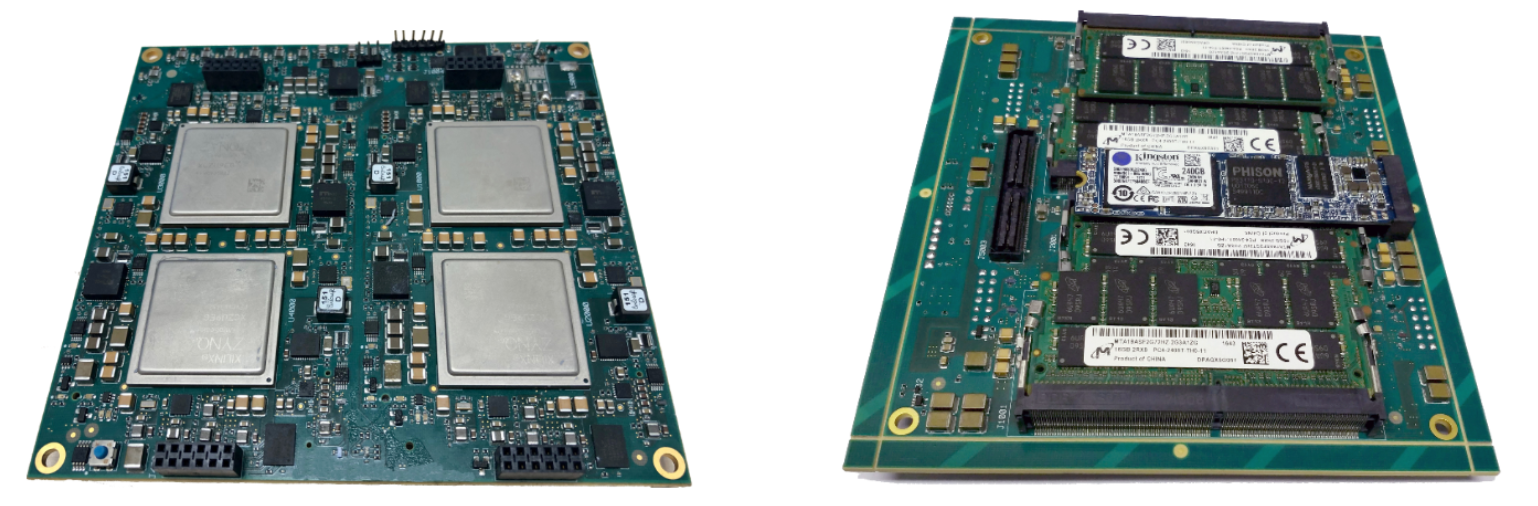
\includegraphics[scale=0.22]{Images/Hardware/QFDB.png}
	% 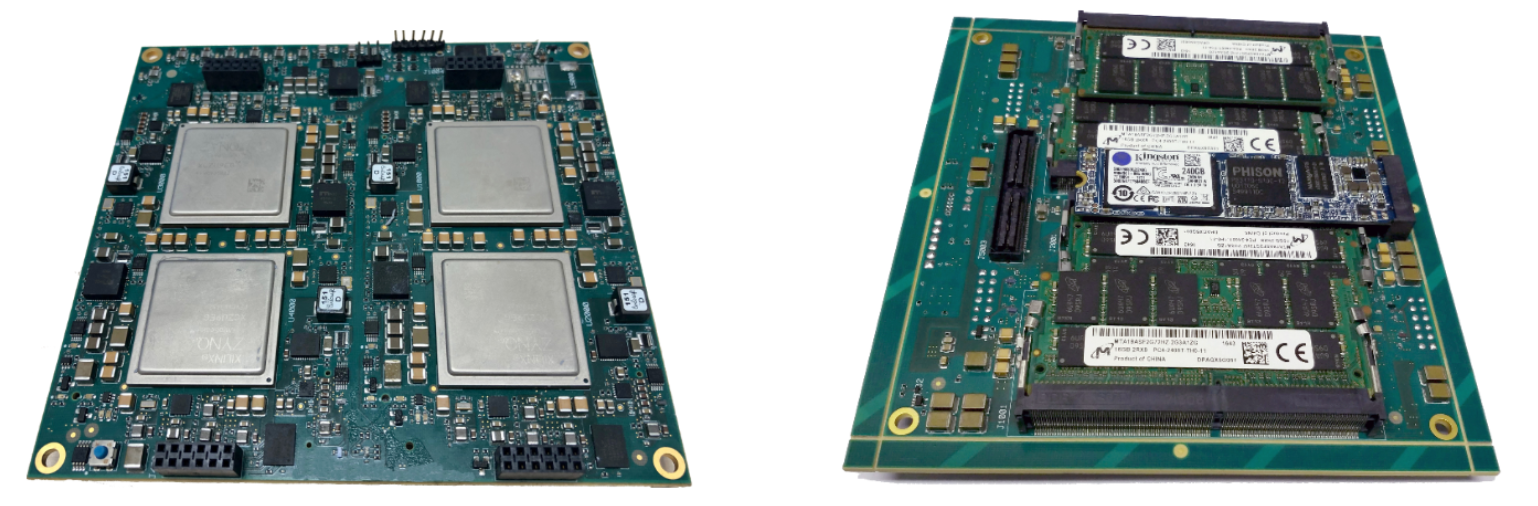
\includegraphics[width=\textwidth]{Images/Hardware/QFDB.png}\\[0.5cm]
	\decoRule
	\caption[FORTH QFDB]{FORTH QFDB, top-view (left) and bottom-view (right): \href{https://ieeexplore.ieee.org/stamp/stamp.jsp?arnumber=8945720}{URL}}
	\label{fig:forth-qfdb-daughterboard}
\end{figure}

In this work, the FPGAs' benefits are being utilized to create a hardware accelerator that can speed up the inference of Convolutional Neural Networks (CNNs), a branch of Deep Neural Networks (DNNs), which is a subfield of Machine Learning.

\section{Scientific Contributions}

\section{Thesis Outline}
% Todo: fill chapter descriptions
\begin{itemize}
	\item \textbf{Chapter 2 - Theoretical Background:} The theoretical background of Machine Learning, with emphasis on Convolutional Neural Networks, is described.
	\item \textbf{Chapter 3 - Related Work:} The related work on the field of Convolutional Neural Networks and their hardware implementations is described.
	\item \textbf{Chapter 4:} Chapter 4 description
	\item \textbf{Chapter 5:} Chapter 5 description
	\item \textbf{Chapter 6:} Chapter 6 description
	\item \textbf{Chapter 7:} Chapter 7 description
\end{itemize}

\chapter{Theoretical Background}

\label{Chapter-Theoretical-Background}

The theoretical background of Machine Learning and Convolutional Neural Networks is being described below.

\section{Machine Learning}
Machine Learning, the name of which was first proposed in 1959 by Arthur Samuel \cite{Some-Studies-in-Machine-Learning-Using-the-Game-of-Checkers}, is a subset of Artificial Intelligence, a Computer Science (CS) field that studies algorithms and statistical models capable of performing specific tasks, such as prediction or decision making, without being explicitly programmed. Instead, sample data are used, also known as "training data", for the machine to "learn" to distinguish useful patterns on the input data capable of creating the needed output, e.g., decision or prediction. There are numerous approaches \cite{Machine-learning-Wikipedia} on the learning algorithms types, as well as on the model types used to get trained.

Such algorithm types, at the time of writing, include, but are not limited to:
\begin{itemize}
	\item \textbf{Supervised Learning:} Algorithms that learn by using "labeled" sample data, data that contain both the inputs and their desired outputs to be used for classification and regression.
	\item \textbf{Unsupervised Learning:} In contrast with the Supervised Learning, unlabeled sample data are used to discover structures that could group or cluster them.
	\item \textbf{Reinforcement Learning:} Algorithms responsible for taking actions in an environment, often also described as software agents, to maximize a specific metric, many of which use dynamic programming techniques.
	\item \textbf{Feature Learning:} Algorithms that by combining or even discarding features from the input samples, try to create a new, more useful set of features. One of the most popular algorithms of this category is Principal Components Analysis (PCA).
	\item \textbf{Anomaly Detection:} Algorithms that try to identify outlier samples, which are characterized by their significant difference compared to the majority of the data used. Such algorithms are often used in noise reduction, data mining, and even security and defense systems.
	\item \textbf{Association Rule Learning:} Algorithms that aim to discover strong relationships between features.
\end{itemize}

Such model types, at the time of writing, include, but are not limited to:
\begin{itemize}
	\item \textbf{Artificial Neural Networks (ANN):} Also known as Connectionist Systems, imitate the biological brain's neural networks.
	\item \textbf{Decision Trees:} Used to make assumptions about the input items' target value (the decision tree's leaves) via its observations (the decision tree's branches). When the target takes continuous values, the Decision Tree is called a Regression Tree.
	\item \textbf{Support Vector Machines (SVM):} Used for classification and regression, most\-ly famous as non-probabilistic, binary, linear classifiers. They can also be used for non-linear classification using the kernel trick.
	\item \textbf{Bayesian Networks:} Represented as directed acyclic graphs, they can include probabilistic relationships.
\end{itemize}

Nowadays, most industries have already used Machine Learning in some sort, indicating the significance and variety of its capabilities. It is estimated \cite{Machine-Learning-Applications} that by the year 2021, AI and ML spending will reach 57.6 Billion USD. Its applications include but are not limited to \cite{Top-Machine-Learning-Applications-in-2019} \cite{Roundup-Of-Machine-Learning-Forecasts-And-Market-Estimates}, web page ranking, image recognition, email filtering, and spam detection, database mining, handwriting recognition, speech recognition, natural language processing, computer vision, image/video/text/speech generation, personalized marketing, traveling, dynamic pricing, healthcare, facial and fingerprint recognition and intrusion detection.

\section{Artificial Neural Network}
It is widely accepted that the brain's most exceptional ability is pattern recognition, which is used to combine "data" from the organism's senses in a way to better understand its environment. Artificial Neural Networks (ANN), a highly popular sub-field of Machine Learning, try to imitate the brain's structure to solve such problems, a structure that has been developing and proving its capabilities for thousands of years.

While ANNs are inspired by biological neural networks, they are not identical. A neural network is a collection of connected neurons, through which electrical signals from sensor organs or other neurons are passed and processed. A biological neuron is comprised of four main parts; Dendrites, Cell body, Axon, and Synaptic terminals (Figure \ref{fig:Standard-structure-of-a-biological-neuron}). A Dendrite and its Dendritic branches are used as the neuron's input, where sensors or other neurons get connected. A neuron can have multiple Dendrites. The neuron's cell body collects all the input signals and applies an "activation" function to create the output signal. Afterward, the output signal is transported through the Axon and then distributed to the next neurons through the Synaptic terminals. The Synaptic terminals to Dendrites connections are called Synapses.

\begin{figure} [H]
	\centering
	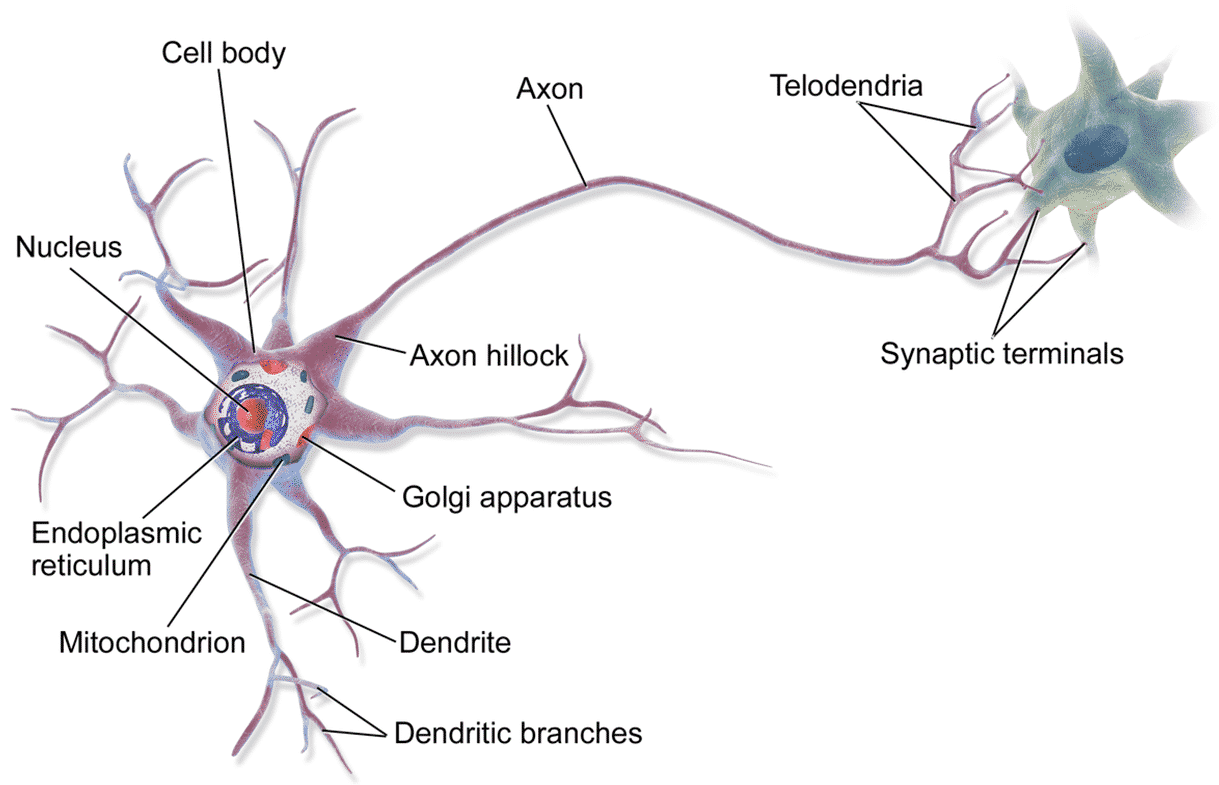
\includegraphics[scale=0.25]{Images/Biological-Neuron.png}
	\decoRule
	\caption[Standard structure of a biological neuron]{Standard structure of a biological neuron: \href{https://nurseslabs.com/nervous-system/}{URL}}
	\label{fig:Standard-structure-of-a-biological-neuron}
\end{figure}

\subsection{ANNs Basic components} \label{subsection:ANNs-Basic-components}
Similarly to the biological neural networks, an ANN can be represented as a directed, weighted graph (Figure \ref{fig:simplified-neural-network-graph}), whose vertices represent the biological neurons' cell bodies and its edges the biological synapses. The electrical signal used in biological neurons can be represented as a real number, and their outputs can be calculated by some non-linear function of the inputs' weighted sum. Each edge typically can have a weight, set during the training process, which amplifies or weakens the vertex's signal.

\begin{figure} [H]
	\centering
	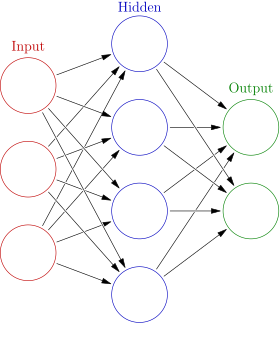
\includegraphics[scale=0.5]{Images/simplified-neural-network-graph.png}
	\decoRule
	\caption[Activation Function Graphs]{Simplified Neural Network Graph: \href{https://en.wikipedia.org/wiki/Artificial_neural_network}{URL}}
	\label{fig:simplified-neural-network-graph}
\end{figure}

\subsubsection{Neuron}
A neuron receives real numbers as inputs, which then using an activation function, are combined with their internal state, also known as activation, and an optional threshold in order to produce the neuron's output.

\subsubsection{Connections and Weights}
Each neuron can be connected with multiple other neurons to be used as inputs and to feed them with its output. Each connection is characterized by its weight, which represents its relative importance.

\subsubsection{Propagation Function}
The propagation function calculates the weighted sum of each neuron's inputs and adds a bias term.

\subsubsection{Activation Function}
The activation function receives the propagation function's result and applies a transformation, which creates the neuron's final output. There are a lot of different activation functions, with specific characteristics for the training and inference process. However, they all provide a smooth and differentiable transition as the input values change. The most commonly used ones are shown below \cite{Activation-Function-Wikipedia}.
\begin{itemize}
	\item \textbf{Identity:} $f(x) = x$\\
	No transformation is applied.

	\item \textbf{Binary Step:} $
		      f(x) =
		      \begin{cases}
			      0 & x \leq 0 \\
			      1 & x > 0
		      \end{cases}
		  $\\
		  While being the original activation function developed when neural networks were invented, it is no longer used as it is incompatible with backpropagation. Backpropagation is the process of updating the weights during the training phase using the gradient descent algorithm. The binary step function is not convex; hence, gradient descent is unable to find a local minimum.

	\item \textbf{Logistic (Sigmoid or Soft step):} $
		      f(x) = \sigma(x) = \frac{1}{1 + e^{-x}}
		  $\\
		  Often used, however, in real-world neural networks, it is avoided due to the vanishing gradient problem \cite{The-Vanishing-Gradient-Problem-During-Learning-Recurrent-Neural-Nets-and-Problem-Solutions}.

	\item \textbf{TanH:} $
		      f(x) = tanh(x) = \frac{e^{x} - e^{-x}}{e^{x} - e^{-x}}
		  $\\
		  Same as Logistic.

	\item \textbf{Rectified Linear Unit (ReLU):} $
		      f(x) =
		      \begin{cases}
			      0 & x < 0 \\
			      x & x > 0
		      \end{cases}
		  $\\
		  The most popular activation function, due to its fast backpropagation speeds, its low penalty on generalization accuracy, and its resistance to saturation conditions \cite{ImageNet-Classification-Using-Binary-Convolutional-Neural-Networks}.

	\item \textbf{Softmax:} $
		      f_i(\textbf{x}) = \frac{
		      e^{x_i}
		      }{
		      \sum_{j=1}^{J}e^{x_j}
		      }
		  $, for i = 1, ..., J\\
		  Commonly used as a final output activation function for multiclass classification. It normalizes the output to [0, 1], and makes the outputs' sum equal to 1. After this transformation, the i-th output's value designates the probability of the input to be the class i.
\end{itemize}

\begin{figure} [H]
	\centering
	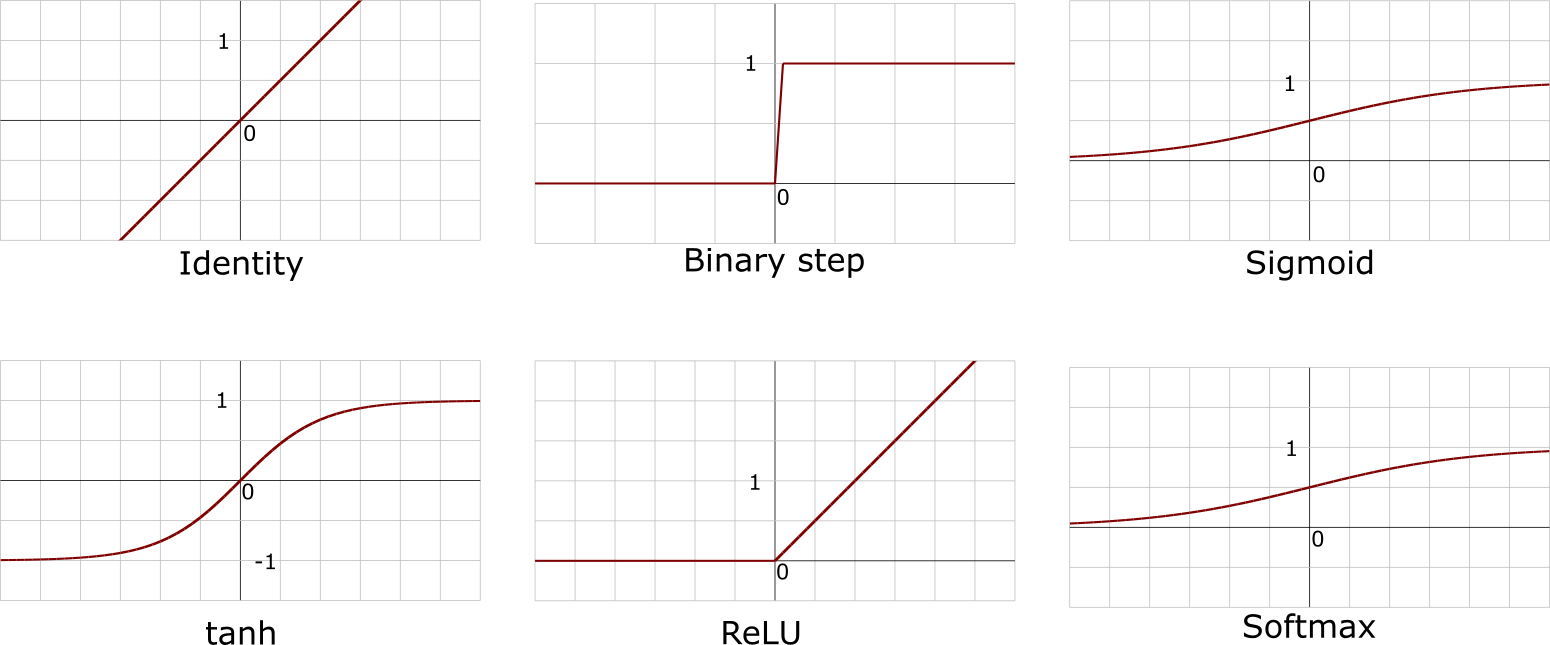
\includegraphics[width=\textwidth]{Images/Activation_functions.png}
	\decoRule
	\caption[Activation Function Graphs]{Activation Function Graphs}
	\label{fig:activation-functions}
\end{figure}

\subsection{Organization}
An ANN's neurons are typically organized into groups, called layers, in which each neuron has the same distance from the inputs as all the other neurons of its group. The input layer is the layer that gets as inputs the external data, and the output layer, the last layer in the graph, is the one that produces the final output results. Any in-between layer is called a hidden layer. An ANN is called a Deep Neural Network (DNN), when, by convention, it has three or more hidden layers.

\subsection{ANN Architectures}
There are many ANN architectures, each one serving different use cases. They are separated into two main groups, Feedforward networks and Recurrent networks \cite{Types-of-Artificial-Neural-Networks}.

\subsubsection{Feedforward Networks}
The basic idea with the feedforward networks is that the data flows from the input layer through the hidden layers to the output layer without any cycles, so they can be represented as directed, acyclic graphs. Some architectures of this group are:
\begin{itemize}
	\item Multiclass Perceptron
	\item Group method of data handling
	\item Autoencoder
	\item Probabilistic
	\item Time delay
	\item Convolutional
	\item Deep stacking network
\end{itemize}

\subsubsection{Recurrent Networks}
Recurrent Neural Networks (RNN), similarly to the Feedforward networks, data flows from the input layer through the hidden layers to the output layer. However, they allow for data cycles, in other words, outputs of the $layer_n$ can be fed to the inputs of the $layer_{n-1}$, so they can be represented as directed, cyclic graphs. Some architectures of this group are:
\begin{itemize}
	\item Fully recurrent
	\item Simple recurrent
	\item Reservoir computing
	\item Long short-term memory
	\item Bi-directional
	\item Hierarchical
	\item Stochastic
	\item Genetic Scale
\end{itemize}
For every ANN Architecture, there are specific types of layers that apply different kinds of mathematical operations on their input data. Each layer type has characteristics on the way its mathematical operations are applied to its input. Those characteristics are generally called hyperparameters. For example, in a Fully-Connected layer, a hyperparameter is its number of outputs. Hyperparameters are set by the engineers during the training phase, which are fine-tuned, concerning the application's input data.

This work is focused on the Convolutional Neural Networks (CNN), which are described in detail below.

\section{Convolutional Neural Networks}
Convolutional Neural Networks (CNNs) are deep feedforward neural networks that specialize in processing data with grid-like topologies and are typically used in visual imagery analysis. They are simple neural networks that, for at least one of their layers, use the convolution mathematical operation instead of the general matrix multiplication \cite{Goodfellow-et-al-2016}.

CNNs imitate the brain's visual cortex, which is the area responsible for the visual processes. Cortical neurons cover small areas of the visual field, with partial overlaps resulting in full visual field coverage.

CNNs most significant advantage over other image classification algorithms is their little need for pre-processing, meaning that their filters are learned during the training phase while using traditional algorithms, they have to be hand-engineered.

Some of their applications are image and video recognition, image classification, object detection, recommendation systems, medical image analysis, natural language processing, and financial time series \cite{Convolutional-neural-networks-wikipedia}.

\subsection{Structure}
A typical CNN consists of two parts. The first part includes multiple convolutional and pooling layers, which extract features from the given input. The second part, also known as the classifier, includes multiple fully connected layers, which classify the given input using the features extracted from the first part (Figure \ref{fig:typical-cnn-architecture}).

\begin{figure} [H]
	\centering
	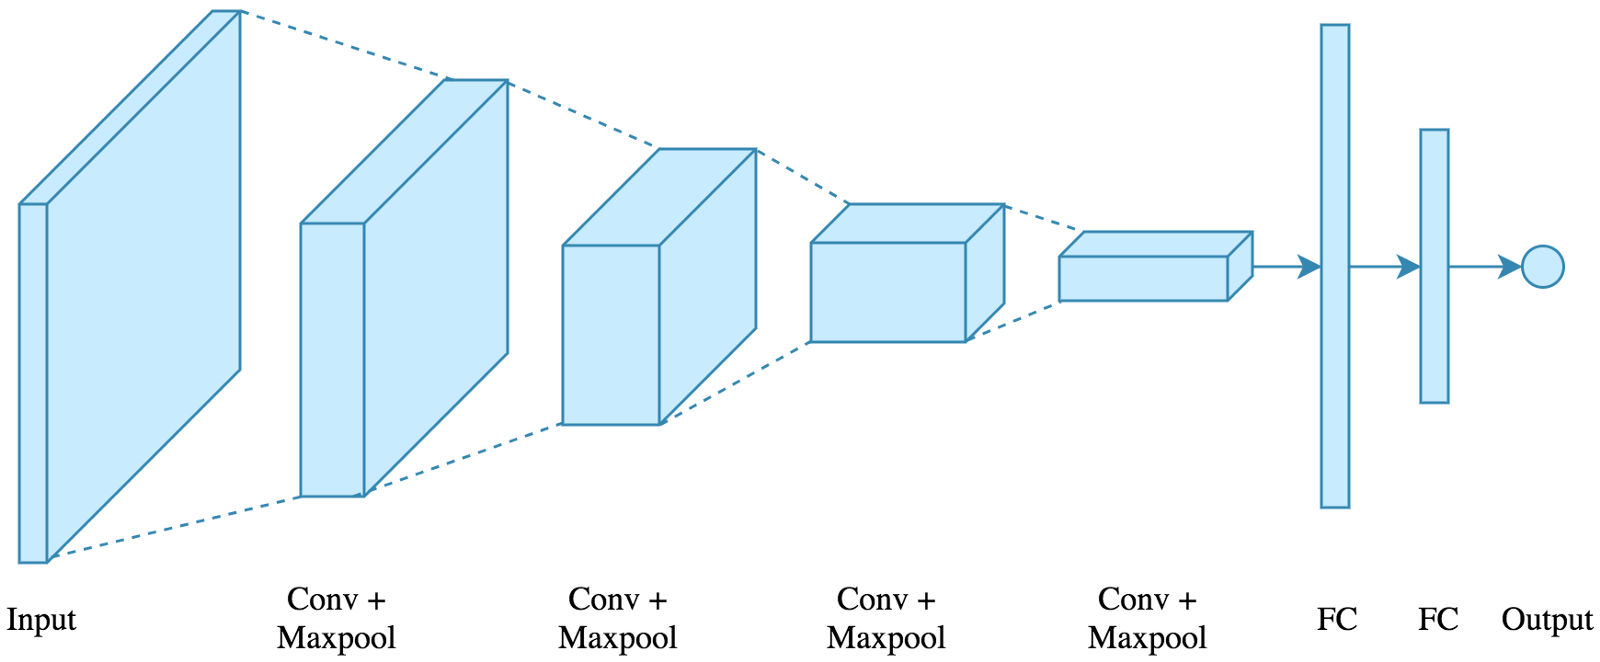
\includegraphics[width=\textwidth]{Images/typical-cnn-architecture.png}
	\decoRule
	\caption[Typical CNN Architecture]{Typical CNN Architecture - First five layers (Convolution + Max Pooling layers) used for feature extraction, last three layers (Fully-Connected) used for classification, also called the classifier: \href{https://www.kaggle.com/mauddib/digit-recogniser-tutorial-using-a-cnn-tensorflow}{URL}}
	\label{fig:typical-cnn-architecture}
\end{figure}

The input data is typically structured as multidimensional arrays, also known as tensors. For example, if the input data are RGB images, then the input tensor's shape is (number of images) x (image width) x (image height) x (image depth), where image depth is called the image's color channels, in this example 3 channels. Moreover, the input data can also be grayscale images or even hyperspectral images. Hyperspectral images have multiple color channels, even in the non-visible for the human eye spectrum, with applications including the medical and space fields. There are also implementations such as 1D and 3D CNNs, but this work examines 2D CNNs only.

The trainable parameters (weights and biases) needed for the computation are initially assigned random values \cite{Practical-recommendations-for-gradient-based-training-of-deep-architectures}, rendering the network useless. However, during the training phase, using the backpropagation process \cite{Learning-internal-representations-by-error-propagation}, those weights are being optimized to form features from the training set. The trainable parameters are also considered to be shared \cite{Generalization-and-network-design-strategies}, meaning that the same parameters are to be used in the entirety of the input data, dramatically decreasing their number and consequently their memory footprint and also increasing the network robustness against overfitting.

As stated above, there are three types of layers used in 2D CNNs; Convolutional, Pooling, and Fully-Connected layers. Each layer is being described below.

\subsubsection{Convolutional Layer}
A convolutional layer creates and outputs a similarity map between the input data and the convolution's filters, also known as kernels. More specifically, every filter is convolved across the input's width and height, producing the dot product of them. The result is multiple two-dimensional arrays, whose each cell holds the similarity of each filter to some spatial position in the input.

Each filter is a specific type of feature, depending on the training set. For example, in image classification, a filter can be a rough shape of cats' mustaches, so that after the convolution, it can be indicated if they are contained somewhere in the input image. If they are, then, to some probability defined during the training phase, there might be a cat in the input image.

Each convolutional layer is defined by its hyperparameters. Those are:
\begin{itemize}
	\item \textbf{Kernel size:} The width and height of the kernels' (filters') size, typically, small\-er than the given input.
	\item \textbf{Output channels:} The number of feature maps to be created as outputs. Consequently, the number of kernels to be used in this operation also equals to the output channels number.
	\item \textbf{Stride:} The number of pixels to be skipped horizontally and vertically in each partial convolution. Typically, this number does not differ between the two dimensions.
	\item \textbf{Zero padding:} There might be a need for zero-padding the input to include as much data as possible in the final computation. There are three different ways of padding:
	      \begin{itemize}
		      \item \textbf{Valid:} No padding is applied; some data may not be included in the computation.
		      \item \textbf{Same:} Applies the amount of padding needed to result in the same width and height as the input.
		      \item \textbf{Full:} Applies padding on the input's edges with a specified number of pixels per dimension.
	      \end{itemize}
\end{itemize}

The mathematical expression of the convolution operation is defined bellow (Equation \ref{eqn:convolution}) and visualized on Figure \ref{fig:convolution-operation}.

Let \emph{I} be the input with \emph{C} channels, \emph{H} height and \emph{W} width, and let \emph{K} be the kernels with \emph{N} number of kernels, \emph{C} channels, \emph{KH} height and \emph{KW} width. Also, let \emph{B} be the bias with K values, and let \emph{S} be the stride size and \emph{P} be the padding size. So the convolution operation's output, \emph{Out}, is defined as:
\begin{equation}
	% Todo: fix overfull hbox
	I_{padded}(c, i, j) = \begin{cases}
		0,                  & i \in [1, P], j \in [1, P]                         \\
		I(c, i - P, j - P), & i \in [P + 1, P + 1 + H], j \in [P + 1, P + 1 + W] \\
		0,                  & i \in [H + 1, H + 1 + P], j \in [W + 1, W + 1 + P] \\
	\end{cases}
\end{equation}

\begin{equation}
	OH = \frac{H + 2P - KH}{S} + 1
\end{equation}

\begin{equation}
	OW = \frac{W + 2P - KW}{S} + 1
\end{equation}

\begin{equation}
	\label{eqn:convolution}
	% Todo: fix overfull hbox
	\begin{split}
		Out(k, i, j) = B(k) +
		\sum_{c = 1}^{C} \sum_{kh = 1}^{KH} \sum_{kw = 1}^{KW}
		I_{padded}(c, kh + i * KH, kw + j * KW) K(k, c, kh, kw),\\
		\mbox{for k = 1, 2, ..., C},\\
		\mbox{for i = 1, 2, ..., OH},\\
		\mbox{for j = 1, 2, ..., OW}\\
	\end{split}
\end{equation}

\begin{figure} [H]
	\centering
	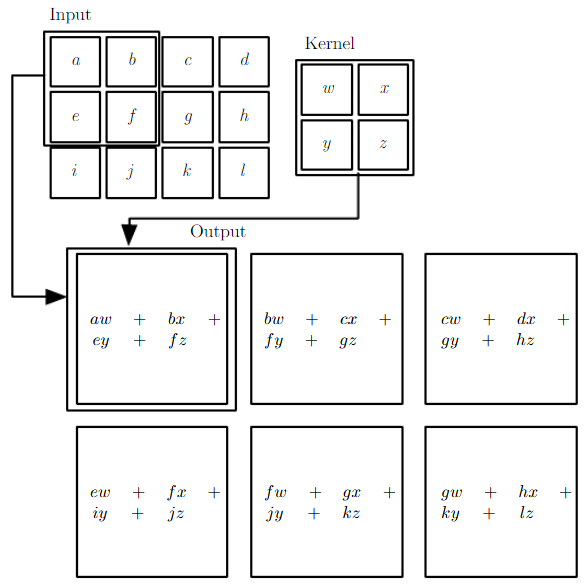
\includegraphics[scale=0.6]{Images/CNNArchitectures/convolution-operation.png}
	% 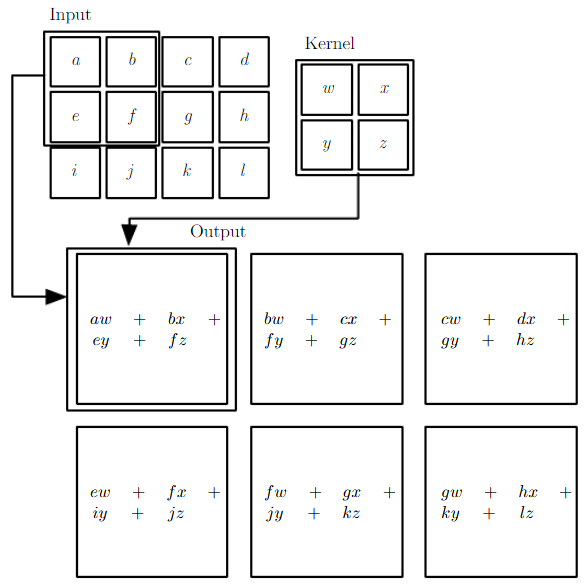
\includegraphics[width=\textwidth]{Images/CNNArchitectures/convolution-operation.png}
	\decoRule
	\caption[Convolution Operation]{Convolution Operation - A 2x2 Kernel filter is applied on the 4x3 example input matrix with stride 1 and valid padding. Figure from \cite{Goodfellow-et-al-2016}.}
	\label{fig:convolution-operation}
\end{figure}

Nowadays, most applications might require multiple Convolutional layers to extract useful features from their complex inputs. Deeper architectures, in general, create more detailed characteristics. Furthermore, activation functions can be interjected between adjacent Convolutional layers to enhance the network's nonlinearity. Activation functions can make the network function as a universal function approximator \cite{Approximation-capabilities-of-multilayer-feedforward-networks}.

\subsubsection{Pooling Layer}
A pooling layer sub-samples its input not only to decrease the computation footprint needed for the next layer, but also to make the network more prone to over-fitting. It reduces the input dimensions by combining multiple neurons into a single neuron. Max-Pooling layers combine groups of neurons by outputting their maximum value. Average-Pooling layers combine groups of neurons by outputting their average value.

Similarly to the convolutional layer, a pooling layer slides a window of some size, called kernel size, across the input data. The data to be combined are those that the sliding window has selected. In 2D CNNs, the pooling layers have 2D windows; the channels are not combined.

A pooling layer can be local, combining small groups of neurons, which also means that the layer's kernel size is small compared to the input size. It can also be global, combining the whole input to a single neuron.

Each pooling layer is defined by its hyperparameters. Those are:
\begin{itemize}
	\item \textbf{Kernel size:} The kernel's (sliding window's) width and height.
	\item \textbf{Stride:} The number of pixels to be skipped horizontally and vertically in each slide. Typically, this number does not differ between the two dimensions.
\end{itemize}

The mathematical expression of the average-pooling operation (Equation \ref{eqn:avg-pooling}) and max-pooling operation (Equation \ref{eqn:max-pooling}) is defined and visualized (Figure \ref{fig:max-pooling-operation}) bellow.

Let \emph{I} be the input with \emph{C} channels, \emph{H} height and \emph{W} width, let \emph{KH} be the kernel's height, let \emph{KW} be the kernel's width, and let \emph{S} be the stride size. So the pooling operations are defined as:
\begin{equation}
	OH = \frac{H - KH}{S} + 1
\end{equation}

\begin{equation}
	OW = \frac{W - KW}{S} + 1
\end{equation}

\begin{equation}
	\label{eqn:avg-pooling}
	\begin{split}
		AvgPool(c, i, j) =
		\frac{
			\sum_{kh = 1}^{KH} \sum_{kw = 1}^{KW}
			I(c, kh + i * KH, kw + j * KW)
		}{
			KH * KW
		},\\
		\mbox{for c = 1, 2, ..., C},\\
		\mbox{for i = 1, 2, ..., OH},\\
		\mbox{for j = 1, 2, ..., OW}\\
	\end{split}
\end{equation}

\begin{equation}
	\label{eqn:max-pooling}
	\begin{split}
		MaxPool(c, i, j) = \max_{1 \leq kh \leq KH, 1 \leq kw \leq KW}
		I(c, kh + i * KH, kw + j * KW),\\
		\mbox{for c = 1, 2, ..., C},\\
		\mbox{for i = 1, 2, ..., OH},\\
		\mbox{for j = 1, 2, ..., OW}\\
	\end{split}
\end{equation}

\begin{figure} [H]
	\centering
	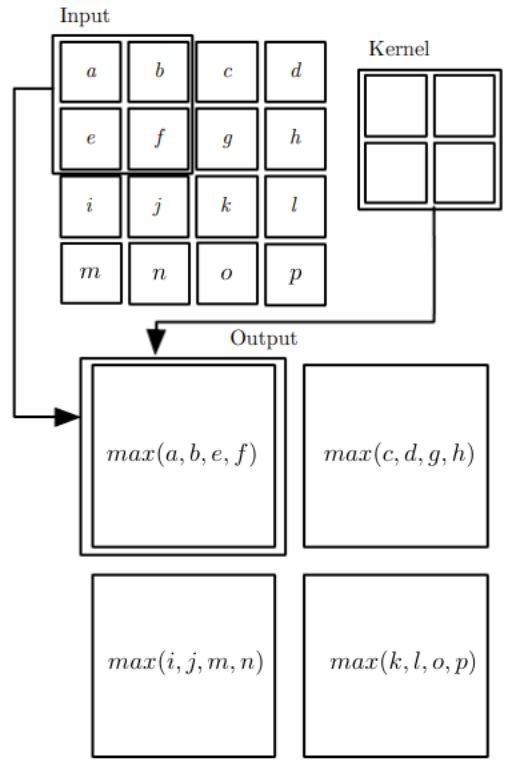
\includegraphics[scale=0.6]{Images/CNNArchitectures/maxpooling-operation.png}
	% 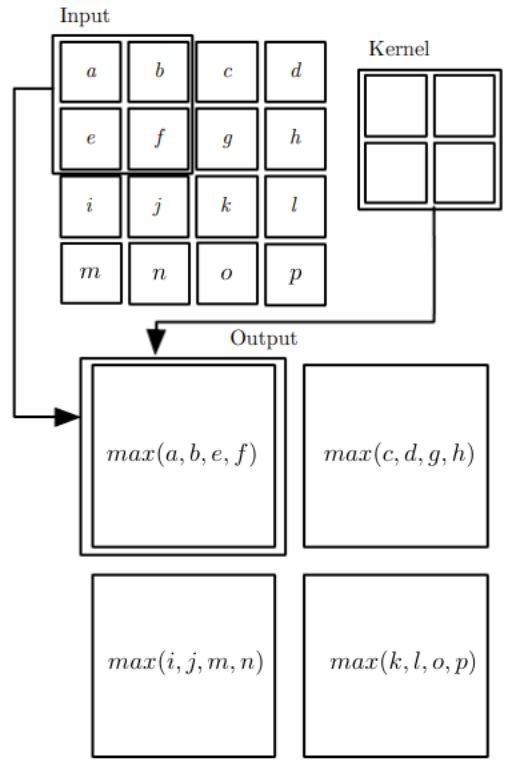
\includegraphics[width=\textwidth]{Images/CNNArchitectures/maxpooling-operation.png}
	\decoRule
	\caption[Max-Pooling Operation]{Max-Pooling Operation - A max operation is applied with a 2x2 Kernel on the 4x4 example input matrix with stride 2. Figure from \cite{Goodfellow-et-al-2016}.}
	\label{fig:max-pooling-operation}
\end{figure}

\subsubsection{Fully-Connected Layer}
The CNNs classifier part is comprised of several Fully-Connected layers, which serve as the high-level reasoning. It is the part that finally classifies the given input.

A Fully-Connected layer is the simplest type of layer, as it is the one used in Multi-Layer Perceptron (MLP) neural networks. More specifically, it receives input, with which it computes a weighted sum for each of its output values. This input is derived from the flattened output of several convolutional and pooling layers.

Each Fully-Connected layer is defined by its hyperparameters. Those are:
\begin{itemize}
	\item \textbf{Output Features:} The number of features to output. Consequently, this also configures the number of weights needed for the computation, hence, its memory and computation footprint.
\end{itemize}

The mathematical expression of the Fully-Connected layer's operation (Equation \ref{eqn:fully-connected}) is defined bellow.

Let \emph{I} be the input with \emph{N} input features, let \emph{W} be the layers weights, let \emph{B} be the layer's bias, and let \emph{M} be the layer's output features. So the Fully-Connected layer's output, \emph{Out}, is defined as:
\begin{equation}
	\label{eqn:fully-connected}
	Out(i) = B(i) + \sum_{j = 1}^{N} I(j)W(i, j), \mbox{for i = 1, 2, ..., M}
\end{equation}

The parameters' reuse of Fully-Connected layers from a specific application to another cannot be done since they are strictly bonded to the classes and high-level features of the particular Convolutional neural network.

The final Fully-Connected layers is typically followed by a Softmax activation layer, which, as stated on section \ref{subsection:ANNs-Basic-components}, it calculates the probability of the input being a certain class. The use of Softmax enables the confidence quantification for every estimation, and easy troubleshooting when the input it misclassified.

\subsubsection{Activation Layer}
After each Convolutional and Fully-Connected layer, there can be an Activation layer, which applies an activation function on the output of its previous layer. An activation layer increases the network's nonlinearity without affecting the convolutional layers' receptive fields. The activation function can be one of those presented in section \ref{subsection:ANNs-Basic-components}, but ReLU and its variants are generally preferred, due to its fast training characteristics and its low penalty on generalization accuracy.

\section{Theoretical knowledge sources}
The aforementioned theoretical background was mostly obtained from the Statistical Modeling and Pattern Recognition course of Electrical and Computer Engineering school at the Technical University of Crete. In addition, the book Deep Learning \cite{Goodfellow-et-al-2016} was used when finer details were needed. Moreover, the Udacity course Intro to Deep Learning with PyTorch by Facebook AI \cite{Udacity-Intro-to-Deep-Learning-with-PyTorch-by-Facebook-AI} was used for a more hands-on approach, focusing on PyTorch and Python in general. Last but not least, a great resource has been all the papers mentioned above.

%\include{Chapters/Chapter3}
%\include{Chapters/Chapter4}
%\include{Chapters/Chapter5}

%----------------------------------------------------------------------------------------
%	THESIS CONTENT - APPENDICES
%----------------------------------------------------------------------------------------

\appendix % Cue to tell LaTeX that the following "chapters" are Appendices

% Include the appendices of the thesis as separate files from the Appendices folder
% Uncomment the lines as you write the Appendices

% Appendix A

\chapter{Frequently Asked Questions} % Main appendix title

\label{AppendixA} % For referencing this appendix elsewhere, use \ref{AppendixA}

\section{How do I change the colors of links?}

The color of links can be changed to your liking using:

{\small\verb!\hypersetup{urlcolor=red}!}, or

{\small\verb!\hypersetup{citecolor=green}!}, or

{\small\verb!\hypersetup{allcolor=blue}!}.

\noindent If you want to completely hide the links, you can use:

{\small\verb!\hypersetup{allcolors=.}!}, or even better: 

{\small\verb!\hypersetup{hidelinks}!}.

\noindent If you want to have obvious links in the PDF but not the printed text, use:

{\small\verb!\hypersetup{colorlinks=false}!}.

%\include{Appendices/AppendixB}
%\include{Appendices/AppendixC}

%----------------------------------------------------------------------------------------
%	BIBLIOGRAPHY
%----------------------------------------------------------------------------------------

% \printbibliography[heading=bibintoc]

\cleardoublepage
\phantomsection
\addcontentsline{toc}{chapter}{References}
\printbibliography[keyword={References}, title={References}]
\printbibliography[keyword={Link}, title={External Links}]

%----------------------------------------------------------------------------------------

\end{document}
